%
%
\section{State-Action Distillation}


In this section, we propose the State-Action Distillation (SAD), an approach for generating the pretraining dataset for ICRL under random policies and random contexts (see Figure~\ref{fig_schematic}).
% We summarize the implementation details of SAD in Algorithms~\ref{alg_collect_context}-\ref{alg_pretrain_deploy}.


As indicated in \eqref{eqn_pretrain_distribution}, the pretraining data consists of the context, the query state and the action label. We start by introducing the generation of the context under random policies in SAD (refer to Algorithm~\ref{alg_collect_context}).
%
It is important to highlight that the context is collected through interactions with the environment under any given random policy (e.g., uniform random policy), and notably, the context not necessarily originates from a complete episode. 
%
These benefits make SAD potentially well-suited for ICRL's real-world applications with random transition data only.
%
\begin{algorithm}
\caption{Collecting Contexts under Random Policy}         \label{alg_collect_context}
\begin{algorithmic}[1]
		\STATE \textbf{Require:} Random policy $\pi$, context horizon length $T$, state space $S$, environment $\tau$, empty context $\ccalC = \emptyset$

        \FOR{$t$ in $[T]$}
            \STATE Sample a state $s \sim S$ and an action $a \sim \pi(\cdot | s)$
            \STATE Collect $(r, s')$ by executing action $a$ in the environment $\tau$
            \STATE Add $(s, a, r, s')$ to $\ccalC$

        \ENDFOR
        \STATE \textbf{Return} $\ccalC$

\end{algorithmic}
\end{algorithm}
%
%
Having collected the random context, we are now in the stage of collecting query states and corresponding action labels for the pretraining of FM under the random policy.


We proceed by recalling that DIT prioritizes the training on high-return pairs from the context data collected. To that end, DIT assigns a weight $w$ to the loss function during the pretraining phase that is proportional to the return-to-go, i.e., 
$w(s_t, a_t) \propto \sum_{t'=t}^T \gamma^{t' - t} r_{t'}.$
% %
% \begin{align}\label{eqn_pseudo_return}
%     w(s_t, a_t) \propto \sum_{t'=t}^T \gamma^{t' - t} r_{t'}.
% \end{align}
% %
Nonetheless, we acknowledge that DIT may not explore to train on good state-action pairs under the random policy for two reasons: ($i$) DIT solely considers to train on the state-action pairs that are observed in the context, which now contains limited and, more importantly, random transition data. 
% and is derived by the random policy.
%
($ii$) Even for the state-action pairs in the collected context, the return-to-go does not necessarily prioritize the optimal pair but rather promotes the pair with high immediate reward, as the discount factor applies starting from the current time step with a horizon of $(T-t+1)$ only, instead of $T$. This issue becomes even more critical in the problems with sparse rewards.
%
% An example is in the sparse-reward MDP problems, where the reward is received solely upon achieving the goal.
% %
% In this case, DIT may consistently focus its learning on the state-action pairs that promise immediate rewards in the (limited) context, rather than thoroughly exploring the entire state and action spaces.
% \blue{I'm still not convinced about this claim. I get that this puts more weight on the $t^\prime =t$, but why is reward 1?} \purple{modified.}


% \blue{I'm not convinced this is needed here. Are we using any of this to define our algorithm? If yes, it is not clear.}
% \purple{I think we do. Here I was trying to say that DIT is not really selecting the optimal action since it only maximizes the immediate reward, while our method aims to select action that maximizes the Q-function.}



% Building upon the limitations of existing SOTA ICRL algorithms, our proposed method SAD aims to generate random contexts and distill the outstanding state-action pairs across the entire state and action spaces as the query state and action label.
% %



Under this circumstance, our SAD approach advocates for distilling the outstanding query states and action labels by searching across the entire state and action spaces under the random policy. 
%
Before proceeding, we recall the definition of the optimal action in the problems of multi-armed bandit (MAB) and MDP. For any query state $s_q$, the optimal action for $s_q$ corresponds to the action that maximizes the optimal Q-function
%
\begin{align}
    &a_\text{MAB}^*(s_q) \overset{\Delta}{=} \argmax_{a \in A} \underbrace{\mbE \left[ r(s_q, a) \right]}_{Q_\text{MAB}^*(s_q, a)}, \quad a_\text{MDP}^*(s_q) \overset{\Delta}{=} \argmax_{a \in A} \underbrace{\mbE_{\pi^*} \!\! \left[ \sum_{t=0}^\infty \gamma^t  r_t | s_0=s_q, a_0=a \right]}_{Q_\text{MDP}^*(s_q, a)},
\end{align}
%
where $s_q$ in the MAB problem refers to the singleton state of bandits, and $\pi^*$ denotes the optimal policy in the MDP.
%
%
However, both $a_\text{MAB}^*$ and $a_\text{MDP}^*$ are intractable to obtain in our problem of interest for two reasons: ($i$) computing the expectation in the Q-function demands to sample infinite episodes; ($ii$) one can only have access to the random policy, instead of $\pi^*$. Therefore, we instead consider ($i$) stochastic approximation that uses the average as the unbiased estimate of the expectation due to the law of large numbers; ($ii$) maximizing the episodic return under the random policy.
%
%
%

\subsection{Trustworthiness of the Random Policy}







Subsequently, the crucial question arises: \textbf{when can we trust the random policy?}
%
We claim: \textit{The random policy is probabilistically trustworthy for the MAB and MDP problems within a trust horizon.}
%
%
We formalize this claim for MAB and MDP in this subsection, which relies on the following assumptions.
%
\begin{assumption}\label{assumption_bound_reward}
   The absolute value of the reward $r(s, a)$ is bounded by a positive constant $B$ for all state-action pairs in the MAB and MDP, i.e., $|r(s, a)| \leq B, \forall (s, a) \in S \times A.$
\end{assumption}
%
%
Note that Assumption~\ref{assumption_bound_reward} is common in the literature~\citep{azar2017minimax, wei2020model, zhang2021near}. 
In particular, in the case of finite state-action spaces, it is always possible to design the reward to avoid the possibility of being unbounded.
%
%
%
%
\begin{assumption}\label{assumption_mdp_equal}
    Given a random policy $\pi$, assume that
    \begin{align}
        \argmax_{ a \in A} Q_\text{MDP}^\pi(s_q, a) = \argmax_{a \in A} Q_\text{MDP}^*(s_q, a), \, \forall s_q \in S.
    \end{align}
\end{assumption}


It is worth highlighting first that Assumption~\ref{assumption_mdp_equal} may not hold universally for all MDP problems. In fact, it is unlikely that a random policy and the optimal policy select the same optimal actions for all problems. Nevertheless, we acknowledge that Assumption~\ref{assumption_mdp_equal} does hold in the MDP problems like the grid world navigation where the reward is received only upon achieving the unique goal~\citep{laskin2022context, lee2024supervised, dong2024context}, which fall into the applicable domains of this work. We visualize in Figure~\ref{fig_single_dim_MDP_visualize} a single-dimensional grid world navigation problem as an example. In particular, the action derived from maximizing the return under the random policy becomes equivalent to that guided by maximizing the return under the optimal policy, as the maximal return induced by both policies corresponds to navigating to the goal as quickly as possible. We formalize this in Proposition~\ref{proposition_single_MDP} and provide a theoretical proof and empirical validation (refer to Appendix~\ref{appendix_validate_assump2}). 
%
Although Assumption~\ref{assumption_mdp_equal} holds for the grid world navigation problems considered in this work, it is crucial to point out that Assumption~\ref{assumption_mdp_equal} may not hold for all grid world navigation problems. To this end, we further discuss the validity of Assumption~\ref{assumption_mdp_equal} for the grid world navigation with two sparse rewards  (see Appendix~\ref{appendix_validate_assump2_two_rewards}), and demonstrate that the validity of Assumption~\ref{assumption_mdp_equal} depends on problem-specific factors such as the rewards and the discount factor $\gamma$.
%
%
%
%
\begin{figure}[ht]
    \centering
    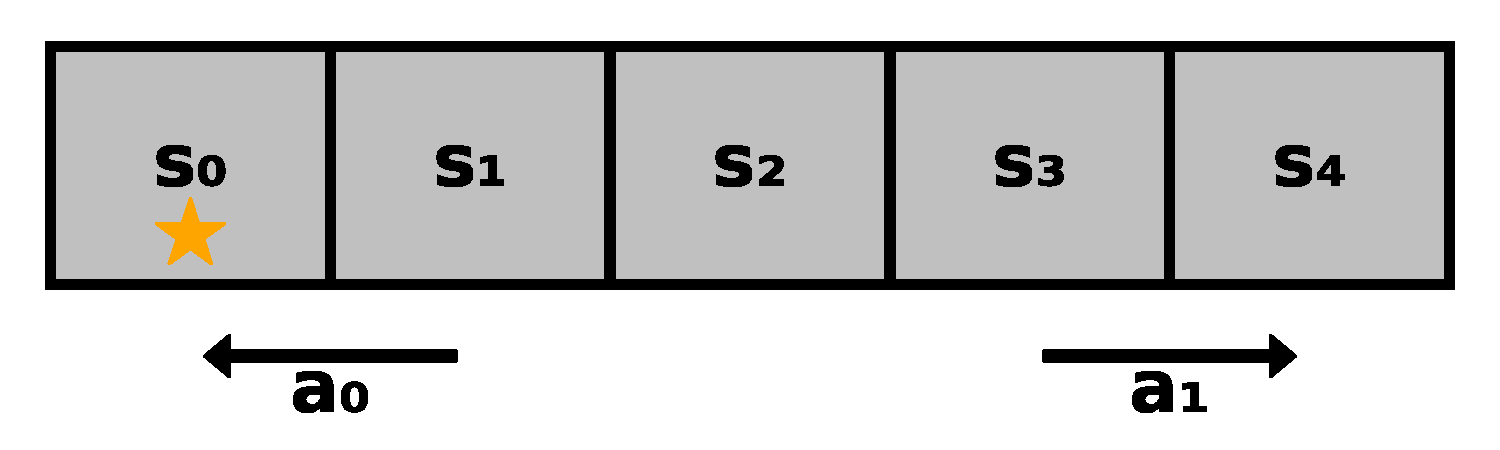
\includegraphics[width=0.35\linewidth]{figures/single_dim_MDP_visualize.pdf}
    \caption{A single-dimensional grid world MDP comprising five states $\{s_0, s_1, s_2, s_3, s_4\}$, where $s_0$ represents the goal state (golden star). The environment offers two possible actions: $a_0$ (go left), and $a_1$ (go right). Any transitions that would result in (left or right) boundary crossing will be confined to the current position. The reward structure is sparse, with a value of 1 received solely upon reaching the unique goal state $s_0$ and a value of 0 otherwise. We consider an infinite time horizon with a discounter factor $\gamma$.}
    \label{fig_single_dim_MDP_visualize}
\end{figure}
%
%
%







Having introduced the necessary assumptions, we are in the stage of investigating the trustworthiness of the random policy in both MAB and MDP problems. To  proceed, we rely on the following two definitions.

\begin{definition}[MAB]\label{definition_mab}
    Denote by $s_q$ and $a^*$ the singleton state and optimal arm in the MAB problem. Consider a random policy $\pi$. Suppose that each arm $a$ has been selected $N_a$ times $(N_a \in \mbN_+)$ under $\pi$. The trustworthiness of the random policy in the the MAB problems represents the probability of selecting the optimal arm under the random policy, i.e., 
    \begin{align}\label{eqn_assump_bandit}
        \frac{1}{N_{a^*}}  \sum_{i=1}^{N_{a^*}} r_i(s_q, a^*) \geq \max_{a \in A \setminus \{a^*\}} \frac{1}{N_{a}} \sum_{i=1}^{N_{a}}  r_i(s_q, a).
    \end{align}
    The corresponding trust horizon denotes the minimal number of selections over all arms, i.e., $N\triangleq \min_{a \in A}  N_a$ that guarantees such trustworthiness.
\end{definition}
%
%
%
%
%
%
%
Definition~\ref{definition_mab} implies by the law of large numbers that $N\to \infty$ serves as a trust horizon, ensuring the selection of the optimal arm with probability one. In practice, achieving large trustworthiness requires a sufficiently large trust horizon. The intuition is that a large enough horizon approximates the infinite step problem. The same intuition holds for the MDP problems.
% \red{Since Assumption~\ref{assumption_mdp_equal} states that the random policy and the optimal policy share the same optimal action in an infinite-horizon MDP, it follows that, in practice, the horizon length of an MDP should be sufficiently long for this equivalence to hold.} 
We formalize this concept in the next definition, which builds upon the Q-function of the finite-horizon MDP
%
% %
% \begin{align}
%     &Q_\text{MDP}^{\pi, N}(s_q, a) = \mbE_\pi \!\! \left[ \sum_{t=0}^{N} \gamma^t r(s_t, a_t) | s_0=s_q, a_0=a \right],\, \forall a \in A.
% \end{align}
% %
\begin{align}
    &Q_\text{MDP}^{\pi, N}(s_q, a) = \mbE_\pi \!\! \left[ \sum_{t=0}^{N} \gamma^t r(s_t, a_t) | s_0=s_q, a_0=a \right],\, \forall a \in A, \\
    &\hat{Q}_\text{MDP}^{\pi, N}(s_q, a) \!=\! \frac{1}{N_\text{ep}} \sum_{i=1}^{N_\text{ep}} \sum_{t=0}^{N} \! \left( \gamma^t r(s_t, a_t) | s_0=s_q, a_0=a, \pi \right),\, \forall a \in A, \label{eqn_Q_mdp_N_hat}
\end{align}
%
where $\hat{Q}_\text{MDP}^{\pi, N}(s_q, a)$ is an unbiased estimate of $Q_\text{MDP}^{\pi, N}(s_q, a)$ and $N_\text{ep}$ denotes the number of episodes.
%
%
\begin{definition}[MDP]\label{definition_mdp}
    Denote by $a^*$ the optimal action given a query state $s_q$. Consider a random policy $\pi$ as well as its Q-function $Q_\text{MDP}^\pi$.
    %
    The trustworthiness of the random policy in the the MDP problems represents the probability of selecting the optimal action for any query state in the state space, i.e.,
    \begin{align}
        \hat{Q}_\text{MDP}^{\pi, N}(s_q, a^*) \geq \max_{a \in A \setminus \{a^*\}} \hat{Q}_\text{MDP}^{\pi, N}(s_q, a), \, \forall s_q \in S.
    \end{align}
    %
    The corresponding trust horizon denotes the minimal horizon length of the MDP such that
    \begin{align}
        Q_\text{MDP}^{\pi, N}(s_q, a^*) \geq \max_{a \in A \setminus \{a^*\}} Q_\text{MDP}^{\pi, N}(s_q, a), \, \forall s_q \in S.
    \end{align}
\end{definition}



% Having introduced the definitions of the trustworthiness and trust horizon. We first formalize the trustworthiness of the random policy for the MAB problem in the following theorem.



In both Definitions~\ref{definition_mab} and \ref{definition_mdp}, the trustworthiness refers to the probability of selecting the optimal action. While the trust horizon in both cases approximates the infinite-horizon problem, they show subtle differences in the relationship to the trustworthiness.
%
% represents the minimum horizon length required for the \red{random policy to select the same optimal actions as the optimal policy}
In the MAB problem, which consists of a single episode, the trustworthiness depends on the trust horizon only. However, in the MDP, computing \( Q_\text{MDP}^{\pi, N}(s_q, a) \) is generally intractable, thus requiring the use of an unbiased estimate (as defined in \eqref{eqn_Q_mdp_N_hat}), which depends on the number of episodes \( N_\text{ep} \). Consequently, the trustworthiness in the MDP setting is influenced by both the trust horizon and the number of episodes. 
%
Next, we formally quantify the relationship between the trustworthiness and the trust horizon for the MAB and MDP problems.



\begin{theorem}[MAB]\label{theorem_mab}
    Let Assumption~\ref{assumption_bound_reward} hold. The random policy is at least $(1-\delta)$-trustworthy as in Definition~\ref{definition_mab}, when the trust horizon $N$ satisfies
    %
    \begin{align}
        N \geq \frac{8B^2}{\left(\mbE[r(s_q, a^*)] - \max\limits_{a \in A \setminus \{a^*\}} \mbE[r(s_q, a)] \right)^2} \log \left( \frac{1+\sqrt{1-\delta}}{\delta} \right).
    \end{align}
\end{theorem}
%
%
%
\begin{myproof}
    See Appendix~\ref{appendix_omit_proof_theorem_mab}.
\end{myproof}
%

% %%%%%%%%%%%%%%%%%%%%%% Bandits %%%%%%%%%%%%%%%%%%%%%%%%%%%%%%%%
% %%%%%%%%%%%%%%%%%%%%%%%%%%%%%%%%%%%%%%%%%%%%%%%%%%%%%%%%%%%%%%%
% %%%%%%%%%%%%%%%%%%%%%%%%%%%%%%%%%%%%%%%%%%%%%%%%%%%%%%%%%%%%%%%
% We start to justify the assumption above by considering the Q-function in the bandits
% %
% \begin{align}
%     &Q (s_q, a) = \mbE \left[r(s_q, a) \right], \, \forall a \in A. \label{eqn_bandit_Q_star} 
%     %\\
%     % &Q_N^\pi (a) = \frac{1}{N} \left(r_1 + r_2 + \cdots + r_N \right), \label{eqn_bandit_Q_pi}
% \end{align}
%
%
% Therefore, it holds by the definition of the optimal arm that
% \begin{align}
%     \max_{a \in A \setminus \{a^*\}} Q(s_q, a) \leq  Q(s_q, a^*).
% \end{align}
% %
% Notice that \eqref{eqn_assump_bandit} represents an empirical version of the previous inequality, and it holds true when the trust horizon $N \to \infty$.
% %



Theorem~\ref{theorem_mab} implies that the trust horizon $N$ quantifies the trustworthiness of the decision making under the random policy $\pi$ for MAB problems. Indeed, a larger $N$ implies a higher probability (smaller $\delta$) that the average reward of the optimal arm under $\pi$ exceeds that of the next-best arm, therefore, making a more reliable decision. We substantiate this claim by empirical evidence (depicted in Figure~\ref{fig_action_select_acc}(a)).
%
%
%
In the practical implementation, we simply execute the MAB under the random policy $\pi$ until every action in the action space $A$ selected at least $N$ times.
%
Subsequently, we select the action with the maximal average reward as the action label. The detailed procedure for collecting such action labels in MAB is outlined in Algorithm~\ref{alg_collect_queries_bandit}.

\begin{algorithm}
\caption{Collecting Query States and Action Labels under Random Policy (MAB)}         \label{alg_collect_queries_bandit}
\begin{algorithmic}[1]
		\STATE \textbf{Require:} Random policy $\pi$, singleton query state $s_q$, action space $A$, environment $\tau$, empty average reward list $L_r$, trust horizon $N$
  
            \STATE Execute the MAB in $\tau$ under the random policy $\pi$ until every action in $A$ selected at least $N$ times
            \FOR{$a$ in $[A]$}
                % \STATE Record the frequency of occurrence $f_a$ of the action $a$ in the history

                \STATE Record the average reward associated with the action $a$ in the history, and add it to $L_r$
            
                % \STATE Compute the average reward by $r_a^{\text{sum}} / N$, and add it to $L_r$

            \ENDFOR

            \STATE Obtain $a_l = A(\argmax (L_r))$

        \STATE \textbf{Return} $(s_q, a_l)$

\end{algorithmic}
\end{algorithm}



% \begin{align}
%     % &Q_\text{MDP}^{\pi, N}(s_q, a) = \mbE_\pi \!\! \left[ \sum_{t=0}^{N} \gamma^t r(s_t, a_t) | s_0=s_q, a_0=a \right], \\
%     &\hat{Q}_\text{MDP}^{\pi, N}(s_q, a) \!=\! \frac{1}{N_\text{ep}} \sum_{i=1}^{N_\text{ep}} \sum_{t=0}^{N} \! \left( \gamma^t r(s_t, a_t) | s_0=s_q, a_0=a, \pi \right),\, \forall a \in A.
% \end{align}
% %
% where $\hat{Q}_\text{MDP}^{\pi, N}(s_q, a)$ is an unbiased estimate of $Q_\text{MDP}^{\pi, N}(s_q, a)$ and $N_\text{ep}$ denotes the number of episodes.
% %





\begin{theorem}[MDP]\label{theorem_mdp}
Let Assumptions~\ref{assumption_bound_reward} and \ref{assumption_mdp_equal} hold.
 Define $\kappa = \min\limits_{s_q \in S} \big( Q_\text{MDP}^\pi(s_q, a^*) - \max\limits_{a \in A \setminus \{a^*\}} Q_\text{MDP}^\pi(s_q, a) \big)$. Consider the trust horizon $N > \log_\gamma \left( \kappa (1-\gamma)/(2B) \right)-1$. The random policy is at least $(1-\delta)$-trustworthy as in Definition~\ref{definition_mdp}, when the number of episodes $N_\text{ep}$ satisfies
%
\begin{align}\label{eqn_theorem_MDP}
    N_\text{ep}  \geq \underbrace{ \frac{ 2 \left( 1-\gamma^{N+1}\right)^2}{ \left( \kappa \left( 1-\gamma \right) / (2B) - \gamma^{N+1}\right)^2} }_{G_1}   \log \left( \frac{1+\sqrt{1-\delta}}{\delta} \right).
\end{align}
\end{theorem}
%
%
\begin{myproof}
    See Appendix~\ref{appendix_omit_proof_theorem_mdp}.
\end{myproof}
%
% % \red{Comment the assumptions. Of course Assumption 2 may not be true if T is large and N is large. See Figure 6.}
% We now proceed to illustrate that Assumption~\ref{assumption_Q_random_mdp}, as stated above, is not without merit and can be considered reasonable in certain scenarios.
% %
% %
% It is significant to highlight that $\hat{Q}_N^\pi (s_q, a)$ and $Q^*(s_q, a)$ become identical for any $s_q \in S$ and $a \in A$ in the case of a single-step MDP ($T=N=0$).
% % %
% In some problems such as grid world navigation~\citep{laskin2022context}, Assumption~\ref{assumption_Q_random_mdp} is reasonable even when $T$ is not particularly small. Specifically, for the states near the goal, the action derived from maximizing the return under the random policy becomes (nearly) equivalent to that guided by maximizing the return under the optimal policy, as the maximal return induced by both policies corresponds to navigating to the goal.
%


Theorem~\ref{theorem_mdp} implies that the trust horizon $N$ and the number of episodes $N_\text{ep}$ quantify the trustworthiness of the decision making under the random policy $\pi$ for MDP problems. Notice that $G_1$ in \eqref{eqn_theorem_MDP} is monotonically decreasing with respect to the trust horizon $N$ when $N > \log_\gamma \left( \kappa (1-\gamma)/(2B) \right)-1$ (see Lemma~\ref{lemma_mono_decrease} in Appendix~\ref{appendix_tech_lemma}). Thus, with a fixed number of episodes, a larger $N$ corresponds to a higher probability (smaller $\delta$) that the average reward of the optimal action under $\pi$ exceeds that of the next-best action, indicating a more reliable decision.
%
%
This aligns with the intuition that a larger $N$ corresponds to a closer approximation of the infinite-horizon MDP, where the random policy $\pi$ selects the same optimal action as that of the optimal policy (by Assumption~\ref{assumption_mdp_equal}).
%
However, it is worth noting that Theorem~\ref{theorem_mdp} considers the worst-case guarantee of selecting the optimal actions over all states in the state space. It is therefore could be conservative. That being said, Theorem~\ref{theorem_mdp} still hints to the fact that one should select the action that yields the largest average reward in practice.
%
%
In the practical implementation, we randomly select a query state from the state space and execute an episode of $N$ steps for each action in the action space. When the maximal return across all actions is no less than a pre-designed return threshold $\mathfrak{R}$, we choose the action that maximizes $\hat{Q}_\text{MDP}^{\pi, N}(s_q, a)$ across the entire action space $A$. Otherwise, we randomly sample another query state and repeat the process of evaluating each action in a horizon $N$. The implementation details are summarized in Algorithm~\ref{alg_collect_queries_dense}.
%
%





\begin{algorithm}
\caption{Collecting Query States and Action Labels under Random Policy (MDP)}
\label{alg_collect_queries_dense}
\begin{algorithmic}[1]
%
		\STATE \textbf{Require:} Random policy $\pi$, state space $S$, action space $A$, environment $\tau$, trust horizon $N$, return threshold $\mathfrak{R}$

        \STATE \textbf{Set} $\texttt{max\_return} = \mathfrak{R} - 1$

        \WHILE{ $\texttt{max\_return} < \mathfrak{R}$ }

            \STATE Sample a query state $s_q \sim S$
            \STATE Empty a return list $L_r$
            \FOR{$a$ in $[A]$}
                \STATE Initialize the state and action as $s_0 = s_q, \, a_0 = a$
            
                \STATE Run an episode of $N$ steps in $\tau$ under the random policy $\pi$
          
            \STATE Add the discounted episodic return to $L_r$

            \ENDFOR
            \STATE $\texttt{max\_return} = \max (L_r)$
        \ENDWHILE
            \STATE Obtain $a_l = A(\argmax (L_r))$

        \STATE \textbf{Return} $(s_q, a_l)$
%
\end{algorithmic}
\end{algorithm}






Notably, this work focuses on the grid world navigation problems where the reward is received solely upon reaching the unique goal. In this sparse reward MDP, it is worth highlighting that the action that maximizes the discounted return is essentially the same as that reaches the goal using fewest steps. This is because that the discounted return $\sum_t \gamma^t r_t$ has a term $\gamma^t$ where $t$ is the time step. Thus, fewer steps (smaller $t$) corresponds to larger discounted return (larger $\gamma^t$). Therefore, for any query state $s_q$, we prioritize actions that can achieve the goal within $N$ steps, with the actions consuming fewer steps being preferred. If no action can accomplish the goal within $N$ steps, we sample another query state until a qualified action is identified. This action is then designated as the action label associated with the query state $s_q$. Details of this implementation are outlined in Algorithm~\ref{alg_collect_queries_sparse} (see Appendix~\ref{appendix_implement}).





















Having introduced the processes for collecting the context, query state, and action label under the random policy, we can now generate the pretraining dataset by integrating the aforementioned procedures (refer to Algorithm~\ref{alg_sad}).
%
Given the pretraining dataset, the model pretraining procedure as well as the offline and online deployment for SAD are summarized in Algorithm~\ref{alg_pretrain_deploy} (see Appendix~\ref{appendix_implement}).

% \purple{
% We note that SAD and DIT has an optimization step for action selection while AD and DPT does not under the random policy.
% }








\begin{algorithm}[ht]
\caption{State-Action Distillation (SAD) under Random Policy}         
\label{alg_sad}
\begin{algorithmic}[1]
		\STATE \textbf{Require:} Empty pretraining dataset $\ccalD$ with size $|\ccalD|$, pretraining environment distribution $\ccalT_{\text{train}}$, random policy $\pi$, context horizon length $T$, state space $S$, action space $A$, trust horizon $N$
        \FOR{$i$ in $[|\ccalD|]$}
            \STATE Sample an environment $\tau \sim \ccalT_{\text{train}}$

            \STATE Collect the context $\ccalC$ under the environment $\tau$ and the random policy $\pi$ through Algorithm~\ref{alg_collect_context}

            \STATE Collect the query state $s_q$ and the action label $a_l$ under the environment $\tau$ and the random policy $\pi$ through Algorithm~\ref{alg_collect_queries_bandit} for MAB (Algorithm~\ref{alg_collect_queries_dense} for MDP)

            \STATE Add $(\ccalC, s_q, a_l)$ to the pretraining dataset $\ccalD$
        \ENDFOR

        \STATE \textbf{Return} $\ccalD$
\end{algorithmic}
\end{algorithm}











\subsection{Performance Guarantees}


This subsection establishes the performance guarantees of SAD, offering deeper insights into its efficacy.
%
%
%
\begin{corollary}
\label{corollary_ps_sampling}
Let hypotheses of Theorems~\ref{theorem_mab}  and \ref{theorem_mdp} hold. Denote by $l$ the length of the trajectory.
For any environment $\tau$ and history data $H$, SAD and the well-specified posterior sampling follow the same trajectory distribution with probability $(1-\delta)^l$
\begin{align}
    P_{\ccalF_{\theta}} (\text{trajectory}  \mid  \tau, H) = P_{ps}(\text{trajectory} \mid \tau, H), \, \forall \text{trajectory}.
\end{align}
%
\end{corollary}
%
\begin{myproof}
    See Appendix~\ref{appendix_omit_proof_corollary_ps_sampling}.
\end{myproof}
%
Notice that DPT takes the same distribution as that from a well-specified posterior sampling~\citep{lee2024supervised}, which is widely recognized as a provably sample-efficient RL algorithm~\citep{osband2013more}.
%
However, it is crucial to highlight that our SAD approach focuses only on the pretraining dataset generation, while maintaining the same pretraining process as that of DPT. Building upon Theorems~\ref{theorem_mab} and \ref{theorem_mdp} implying that SAD probabilistically selects the optimal action (required by DPT), Corollary~\ref{corollary_ps_sampling} substantiates that our SAD approach follows the same trajectory distribution as that of the posterior sampling with probability $(1-\delta)^l$.



Having established the corollary above, we next investigate the regret bound of SAD in the finite MDP setting (see details in Appendix~\ref{appendix_finite_mdp_setting}).
%
Consider the online cumulative regret of SAD over $K$ episodes in the environment $\tau$ as $\text{Regret}_\tau(\ccalF_{\theta}) = \sum_{k=0}^K V_\tau (\pi_\tau^*) - V_\tau(\pi_k)$, where $\pi_k (\cdot \mid s_t) = \ccalF_{\theta}(\cdot \mid \ccalC_{k-1}, s_t)$.
% \begin{align}
%     \text{Regret}_\tau(\ccalF_{\theta}) = \sum_{k=0}^K V_\tau (\pi_\tau^*) - V_\tau(\pi_k).
% \end{align}
%
Then, the regret bound of SAD is formally stated as follows.
%
\begin{corollary}
\label{corollary_regret_bound}
Let hypotheses of Theorems~\ref{theorem_mab} and \ref{theorem_mdp} hold.
%
Given environment $\tau$ and a constant $B' > 0$, suppose that $\sup_{\tau} {\ccalT_{\text{test}}(\tau)}/{\ccalT_{\text{train}}(\tau)} \leq B'$. In the finite MDP with horizon $T$, it holds with probability $(1-\delta)^{KT}$ that
\begin{align}
       \mbE_{\ccalT_{\text{test}}} \left[ \text{Regret}_\tau(\ccalF_{\theta}) \right]  \leq \widetilde{\ccalO} (B' |S| T^{3/2} \sqrt{K |A|}). \label{eqn_regret_bound}
\end{align}
%
\end{corollary}
%
\begin{myproof}
    See Appendix~\ref{appendix_omit_proof_corollary_regret_bound}.
\end{myproof}
%
Analogous to Corollary~\ref{corollary_ps_sampling}, Corollary~\ref{corollary_regret_bound} implies that SAD achieves the same regret bound as that of DPT (\eqref{eqn_regret_bound}) with probability $(1-\delta)^{KT}$, as SAD and DPT undergo the identical pretraining process.













%%%%%%%%%%%%%%%%%%%%%%%%%%%%%%%%%%%%%%%%%%%%%%%%%%%%%%%%%%%%%%%%%%%%%%%%
